本实验以同一个 10\,MHz 时钟为被测信号，比较 100\,MHz 和 200\,MHz 两种 ILA 采样频率对边沿时间分辨率及记录时长的影响。

\subsection{实验过程}
在同一块 FPGA 上，将 10\,MHz 时钟分别接入 \texttt{ila100} 和 \texttt{ila200}。两个 ILA 的采样深度均为 4096 点。在 Hardware Manager 中打开各自的波形页，选取两个相邻上升沿，按横轴样点序号之差换算周期。

\subsection{实验结果}
图~\ref{fig:ex3-ila100} 的活动波形页为 \texttt{hw\_ila\_1}，对应 100\,MHz 采样。每两个相邻上升沿约相隔 10 个样点，其中高电平约占 5 点。采样间隔为 10\,ns，因此测得周期约为 $10\times 10\,\mathrm{ns}=100\,\mathrm{ns}$。

\begin{figure}[H]
    \centering
    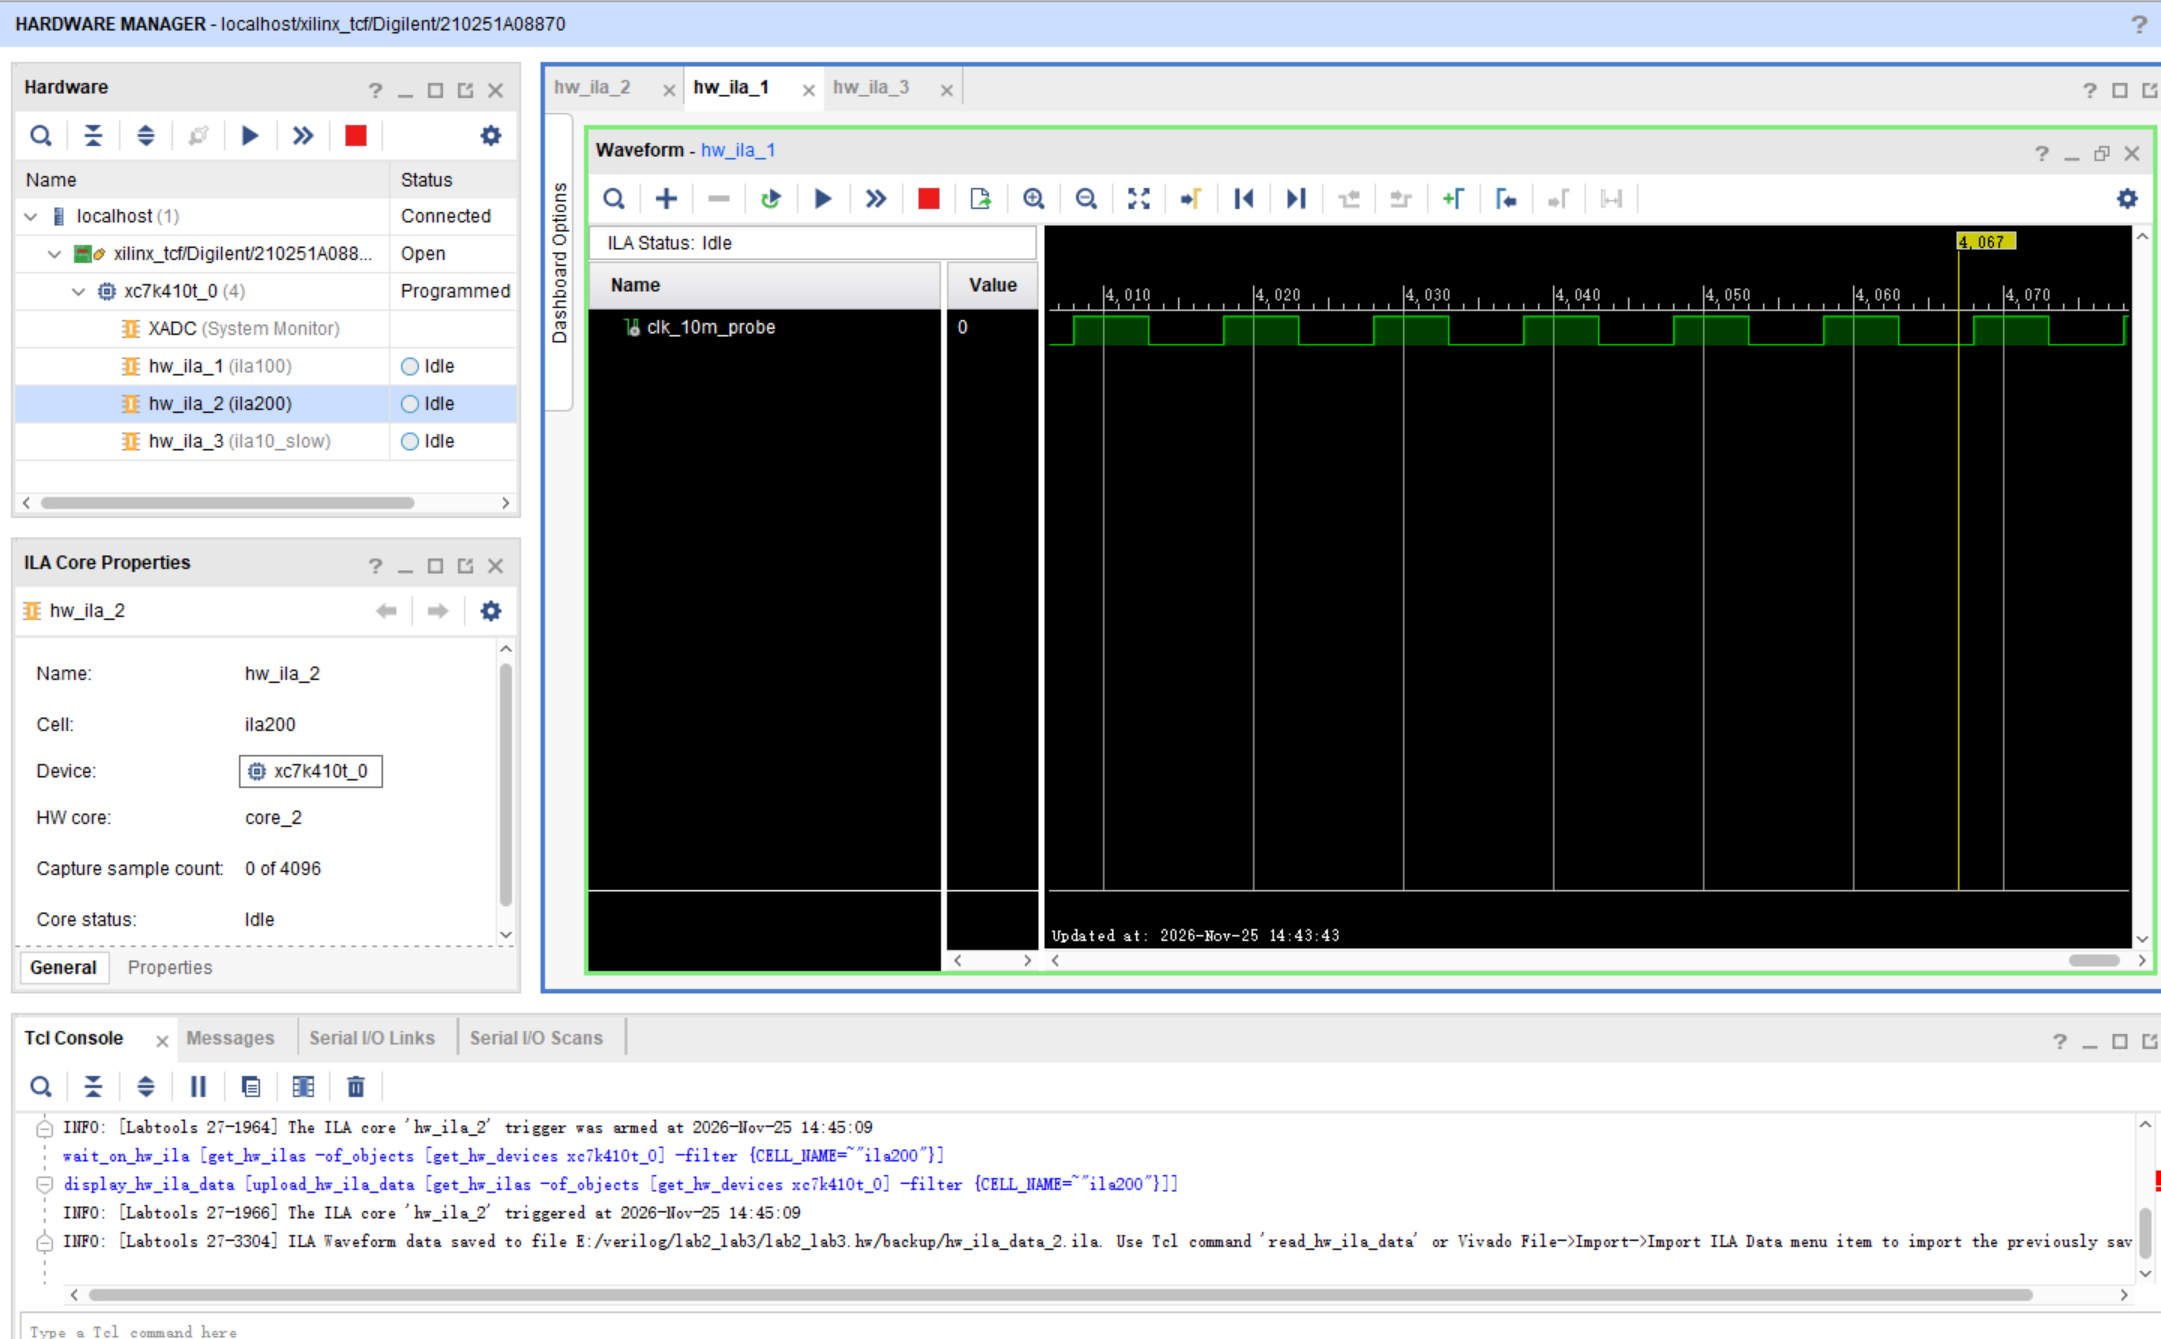
\includegraphics[width=\linewidth]{sections/ex3/picture/board_100mhz.png}
    \caption{100\,MHz 采样下的 10\,MHz 时钟，活动页为 \texttt{hw\_ila\_1}}
    \label{fig:ex3-ila100}
\end{figure}

图~\ref{fig:ex3-ila200} 的第三行是同一信号在 200\,MHz 采样下的记录。此时相邻上升沿约相隔 20 个样点，其中高电平约占 10 点。采样间隔缩短至 5\,ns，换算所得周期仍约为 $20\times 5\,\mathrm{ns}=100\,\mathrm{ns}$。

\begin{figure}[H]
    \centering
    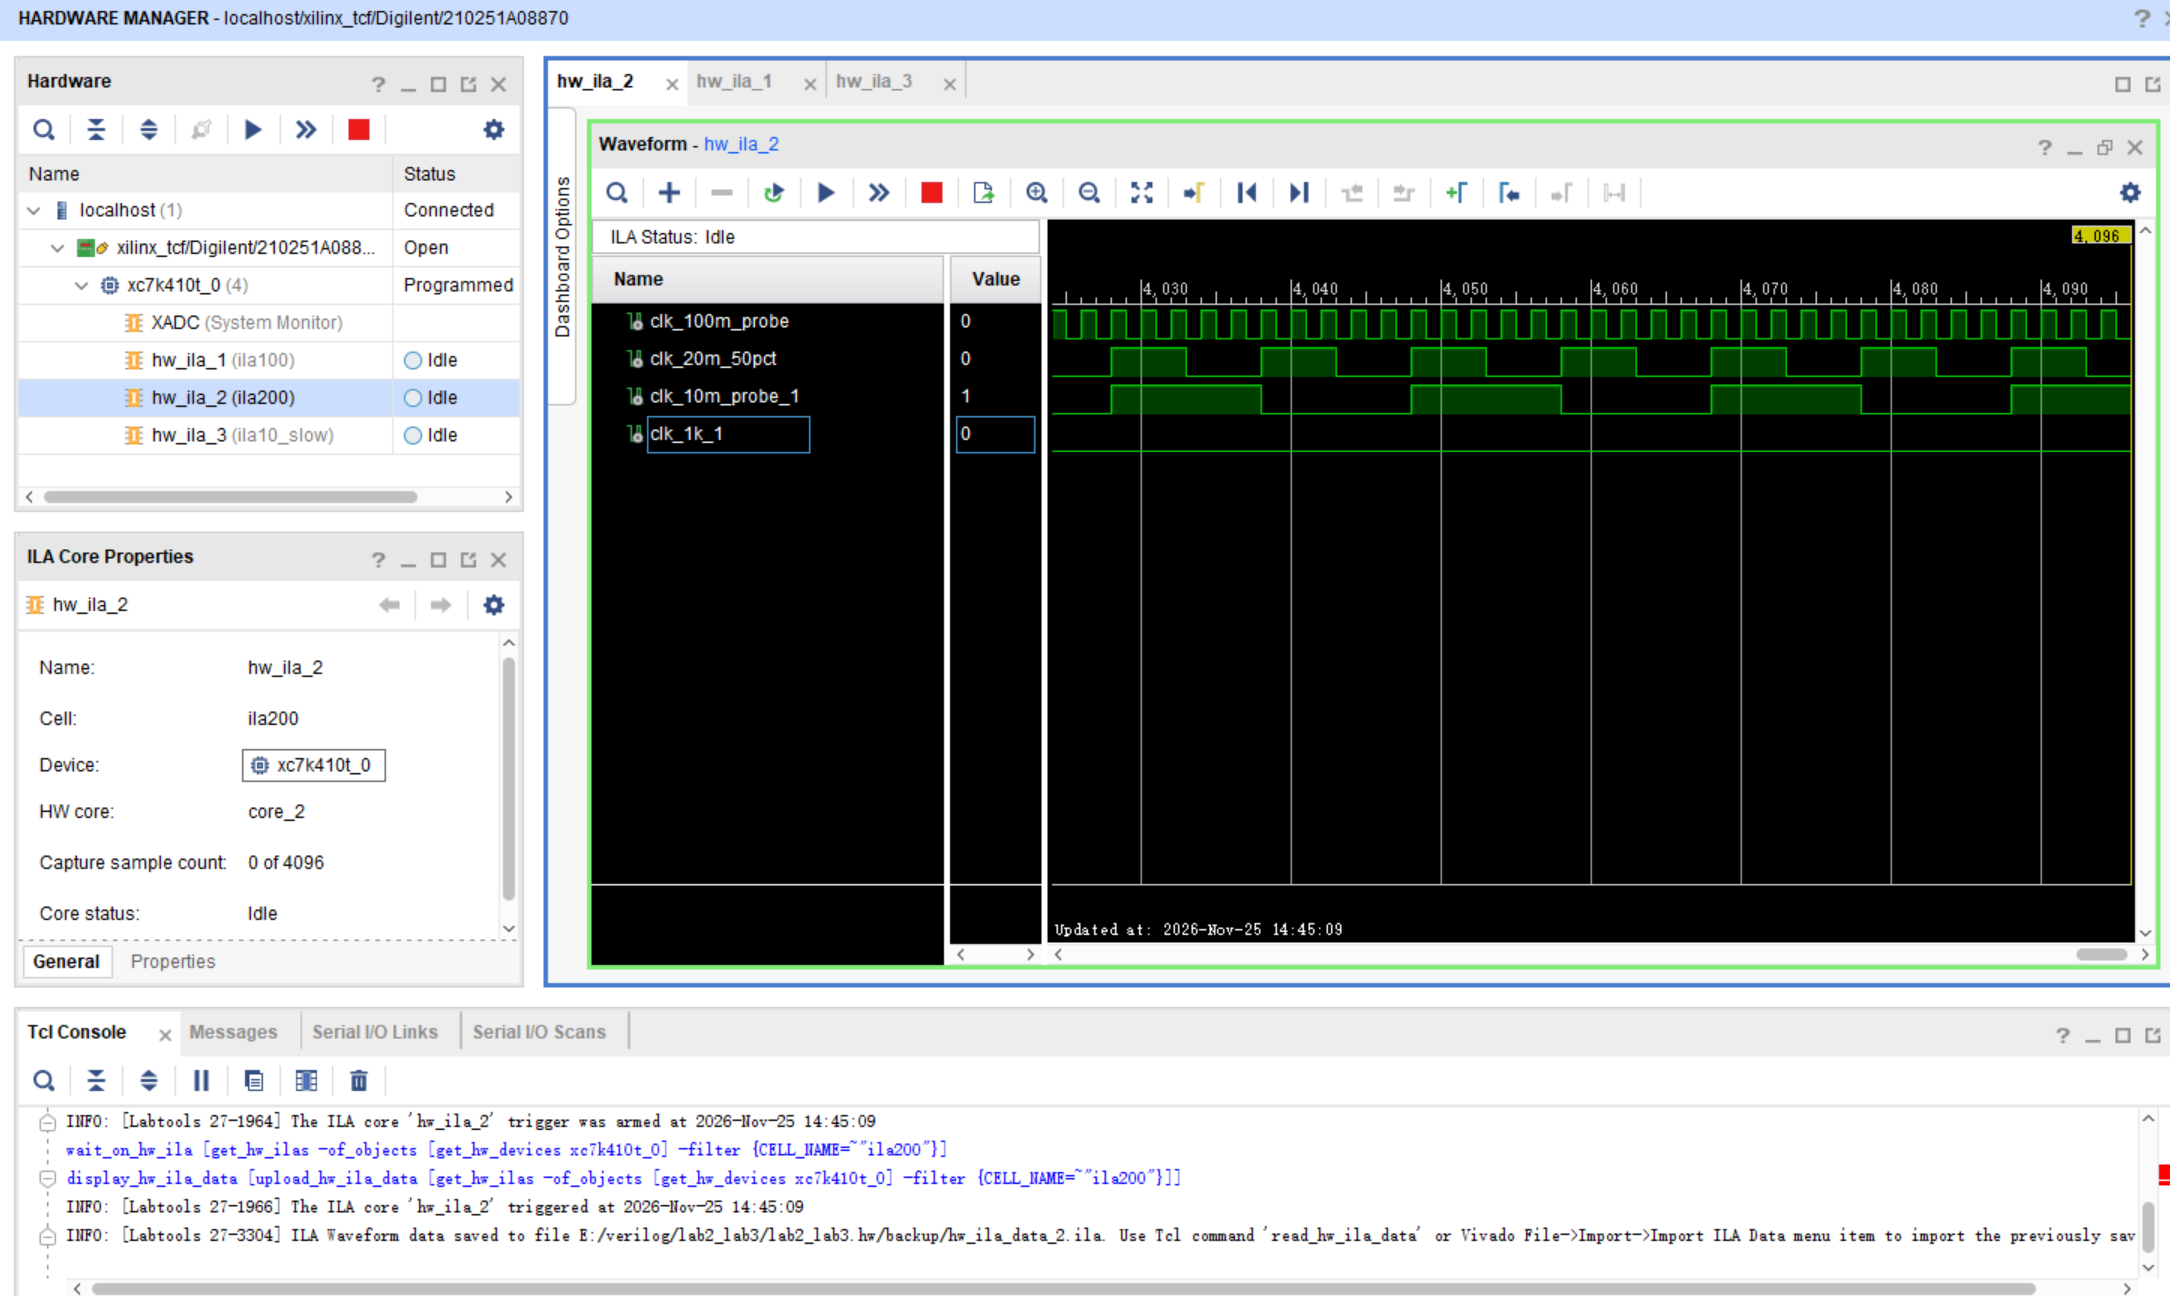
\includegraphics[width=\linewidth]{sections/ex3/picture/board_200mhz.png}
    \caption{200\,MHz 采样下的对照波形，第三行 \texttt{clk\_10m\_probe\_1} 为被测时钟}
    \label{fig:ex3-ila200}
\end{figure}

两次采样均得到约 10\,MHz 的频率和约 50\% 的占空比。采样频率加倍后，每周期的样点数从 10 增至 20，边沿的定位间隔从 10\,ns 缩短到 5\,ns。在同样的 4096 点深度下，记录窗口也从 $40.96\,\mu\mathrm{s}$ 缩短至 $20.48\,\mu\mathrm{s}$。因此，观测快速跳变时可以提高采样频率；若还需覆盖较长时间，则需相应增加采样深度。

\subsection{验收指标}
\begin{enumerate}
    \item 二者的波形差异，边沿刻画程度描述，以及原因介绍
\end{enumerate}
